\subsection{Data Model}
\subsubsection{Data Model and Back-end Structures}
\label{sec:datamodel}

With the overall requirements set we began working on the data model of the system with an initial focus on the database entities and relationships. The database entity-relationship model was sketched in LucidChart using the notation from Database Management Systems \cite{dbbook}. The complete E-R  model is shown below.

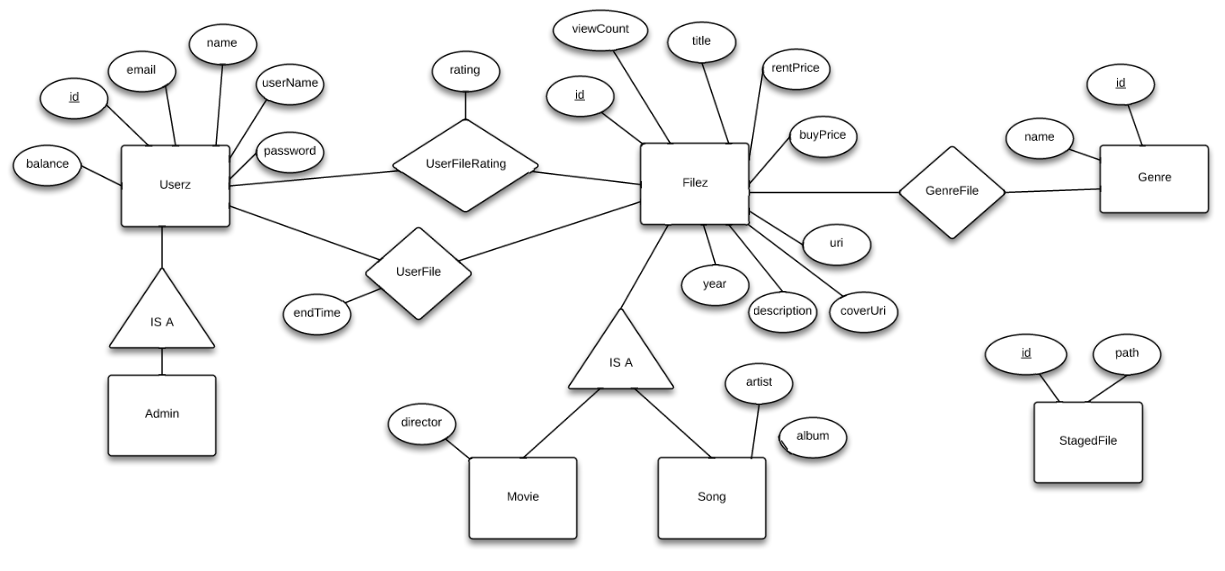
\includegraphics[scale=0.5]{./p2Communication/erdmodel.png}

\subsubsection{Reading the ER-model}
\label{sec:readingdatamodel}
Our design follows a naming scheme, where each table is named after the real domain object it represents, with junction tables following the structure\linebreak <table1><table2><optional own name>.
This structure caused a problem with the “User” and “File” tables, since these names are reserved keywords in MS SQL. We updated said tables by appending a ‘z’ to the name, but we did not update the junction tables.

\subsubsection{Normalization}
\label{sec:normalization}
Besides creating a database structure capable of holding all the data needed for our use cases, we wanted to avoid redundant data. Our choice to avoid redundant data stems from the wish to eliminate anomalies within the database of which redundant data is a key cause. Anomalies are known to weaken the integrity of the database \cite{dbbook} due to irregular or inconsistent data, and we believe integrity is a key characteristic of a database dealing with users, their money, and their property. We enforced this constraint by applying a database normalization (third normal form) to our design, which is known to be free of update, insertion, and deletion anomalies.

\subsubsection{Designing for Extendability}
\label{sec:extendability}
During the design of our entity relationship model, we took time to brainstorm how the design might evolve during the lifespan of the product and how the datamodel might accommodate to those changes. We settled on two plausible cases
\begin{itemize}
\item A need for several types of medias
\item A need for several types of user roles
\end{itemize}
In the following we will explain how we designed for extendability in the context of the first case, but the principle applies to them both.
The naïve solution would be to create a new table for each media type e.g. 
\textbf{Song (id, title, artist, album, coverURI, rentPrice, …)} or
\textbf{Movie (id, title, director, coverURI, rentPrice, …)}
This will however create a lot of duplicate columns in different tables. If we wanted to add new information to our media types later, e.g. a “viewCount” (which did actually happen) this would need to be added to every media table.
The realization that several columns of information is shared across the media suggest for an inheritance based approach, where the shared columns are placed in a “super table”, while every media table will take part in an IS-A relationship with said “super table”.

This design can be seen in our final entity relationship model.

\subsubsection{Improvements}
\label{sec:improvementsdatamodel}
Looking back at our database design we realized that a few improvements could be made. We have sketched these below:
\begin{itemize}
\item Currently our movie table has a director property while our song table has an artist property. These could be moved into the File(z) table with the name “creator”.
\item Our current design does not support several directors/artists. This could have been designed like we designed the genres.
\end{itemize}

\subsubsection{Accessing the Database}
\label{sec:databaseaccess}
After having designed the database structure we had to decide how to access and utilize the database in the best suited way for our webservice. We quickly settled for a C\#/WCF-based web service, since every group member had about the same experience in that platform from other ITU courses.
With access to the .NET framework, we considered to make use of the Entity Framework for our database interactions and general object-relational mapping. However several group members had been experiencing some inconvenient performance issues in previous projects. We do believe performance is an important aspect of our service and research has shown that users of the internet have become very impatient with regards to response times \cite{webusersflee}. We also deemed our queries and database interaction to be fairly simple, thus having no real need for most of the functionality in the Entity Framework. After a discussion it became clear that the only real benefit of using the framework was the possibility of faster prototyping. With our emphasis on a solid performance we choose to spend a little more time developing our own database access layer in order to maintain a more direct control over the performance of our solution.

\subsubsection{Other Potential Sections}
\textbf{Nævn lazy loading?}
Vi bruger det sådan set ikke til noget meget smart

\textbf{Mulige arbejdsgange/forespørgsler understøttet}
Voldsomt ligegyldigt? Alle use cases er jo understøttet. Kan ikke se noget at skrive her.

\textbf{Hvordan ER-diagram mappet til C\# objekterne, ala User -> userobjekt..}
Rimelig selvforklarende mapning vi bruger. De fleste entities hedder det samme.
